% \date{May 14, 2024}
% \author{Deralive}
% \title{华东师范大学软件学院实验报告模板}
% 注意事项:编译两次,以确保目录、页码完整显示

\def\allfiles{}

%————————————多文件编译————————————%
% \ifx\allfiles\undefined
% 	    \begin{document}
% \else
% \fi

% Content

% \ifx\allfiles\undefined
% 	    \end{document}
% 	\else
% 	\fi
%—————————————————————————————————%

\documentclass[14pt,a4paper,UTF8,twoside]{article}

\usepackage{amsmath}
\usepackage{graphicx}
\usepackage{geometry} 
\usepackage{ctex}
\usepackage{multicol}
\usepackage{booktabs} % 表格库
\usepackage{titlesec} % 标题库
\usepackage{fancyhdr} % 页眉页脚库
\usepackage{lastpage} % 页码数库
\usepackage{listings} % 代码块包
\usepackage{xcolor}
\usepackage[hidelinks]{hyperref}
\usepackage{tikz}
\usepackage{tikz-qtree}
\usepackage{fontspec} % 允许设置字体
\usepackage{unicode-math} % 允许数学公式使用特定字体
\usepackage{mwe}
\usepackage{zhlipsum} % 中文乱数文本
\usepackage{amsmath}
\usepackage{xcolor}
\usepackage{float} % 浮动体环境
\usepackage{subcaption} % 子图包
\usepackage[sorting=none]{biblatex}
\usepackage{array}
\usepackage{multirow}
\addbibresource{references.bib} % 指定你的.bib文件名称

\definecolor{mygreen}{rgb}{0,0.6,0}
\definecolor{mygray}{rgb}{0.5,0.5,0.5}
\definecolor{mymauve}{rgb}{0.58,0,0.82}

\date{} % 留空,以让编译时去除日期

%———————————————注意事项—————————————————%

% 1、如果编译显示失败,但没有错误信息,就是 filename.pdf 正在被占用
% 2、在文件夹中的终端使用 Windows > xelatex filename.tex 也可编译

%—————————————华东师范大学———————————————%

% 论文制作时须加页眉,页眉从中文摘要开始至论文末
% 偶数页码内容为:华东师范大学硕士学位论文,奇数页码内容为学位论文题目

%————————定义 \section 的标题样式————————%

% 注意:\chapter 等命令,内部使用的是 \thispagestyle{plain} 的排版格式
% 若需要自己加上页眉,实际是在用 \thispagestyle{fancy} 的排版格式
% 加上下面这一段指令,就能够让 \section 也使用 fancy 的排版格式
% 本质就是让目录、第一页也能够显示页眉、页脚

\fancypagestyle{plain}{
  \pagestyle{fancy}
}

\title{华东师范大学软件学院课程作业} % 模板
\titleformat{\section}
    {\normalfont\bfseries\Large} % 字体大小、字体系列(\bfseries 为加粗)
    {\thesection}{1em}{}

% 设置章节的中文格式
\renewcommand\thesection{\chinese{section} \hspace{0pt}}
\renewcommand\thesubsection{\arabic{subsection} \hspace{0pt}}
% \renewcommand\thesubsubsection{\alph{subsubsection} \hspace{0pt}} % 字母编号
% \hspace{0pt} 是为了确保在章节编号和章节题目之间不要有空格,使得排版更为美观
    
%—————————————页面基础设置———————————————%

\geometry{left=10mm, right=10mm, top=20mm, bottom=20mm}

%————————————设置页眉、页脚——————————————%

\pagestyle{fancy} % 设置 plain style 的属性

% 设置页眉

\fancyhead[RE]{\leftmark} % Right Even 偶数页右侧显示章名 \leftmark 最高级别章名
\fancyhead[LO]{\rightmark} % Left Odd 奇数页左侧显示节名 \rightmark 第二级别节名
\fancyhead[C]{华东师范大学软件学院课程作业} % Center 居中显示
\fancyhead[LE,RO]{~\thepage~} % 在偶数页的左侧,奇数页的右侧显示页码
\renewcommand{\headrulewidth}{1.2pt} % 页眉与正文之间的水平线粗细

% 设置页脚:在每页的右下脚以斜体显示书名

\fancyfoot[RO,RE]{\it Lab Report By \LaTeX} % 使用意大利斜体显示
\renewcommand{\footrulewidth}{0.5pt} % 页脚水平线宽度

% 设置页码:在底部居中显示页码

\pagestyle{fancy}
\fancyfoot[C]{\kaishu 第 \thepage 页 \ 共 \pageref{LastPage} 页} % LastPage 需要二次编译以获取总页数

%——————————————代码块设置———————————————%

\lstset {
    backgroundcolor=\color{white},   % choose the background color; you must add \usepackage{color} or \usepackage{xcolor}
    basicstyle=\footnotesize,        % the size of the fonts that are used for the code
    breakatwhitespace=false,         % sets if automatic breaks should only happen at whitespace
    breaklines=true,                 % sets automatic line breaking
    captionpos=bl,                   % sets the caption-position to bottom
    commentstyle=\color{mygreen},    % comment style
    deletekeywords={...},            % if you want to delete keywords from the given language
    escapeinside={\%*}{*},           % if you want to add LaTeX within your code
    extendedchars=true,              % lets you use non-ASCII characters; for 8-bits encodings only, does not work with UTF-8
    frame=single,                    % adds a frame around the code
    keepspaces=true,                 % keeps spaces in text, useful for keeping indentation of code (possibly needs columns=flexible)
    keywordstyle=\color{blue},       % keyword style
    % language=Python,               % the language of the code
    morekeywords={*,...},            % if you want to add more keywords to the set
    numbers=left,                    % where to put the line-numbers; possible values are (none, left, right)
    numbersep=5pt,                   % how far the line-numbers are from the code
    numberstyle=\tiny\color{mygray}, % the style that is used for the line-numbers
    rulecolor=\color{black},         % if not set, the frame-color may be changed on line-breaks within not-black text (e.g. comments (green here))
    showspaces=false,                % show spaces everywhere adding particular underscores; it overrides 'showstringspaces'
    showstringspaces=false,          % underline spaces within strings only
    showtabs=false,                  % show tabs within strings adding particular underscores
    stepnumber=1,                    % the step between two line-numbers. If it's 1, each line will be numbered
    stringstyle=\color{orange},      % string literal style
    tabsize=2,                       % sets default tabsize to 2 spaces
    % title=Python Code              % show the filename of files included with \lstinputlisting; also try caption instead of title
}

% 注释掉的部分用于后续插入代码,参数可调整,格式如下:

% 1、直接插入
% \begin{lstlisting}[language = ? , title = { ? } ]
%       Your code here.
% \end{lstlisting}

% 2、文件插入
% \lstinputlisting[language = C , title = ?.c] {filename.c}

%———————————————字体设置————————————————%

% \setCJKmainfont{SimSun} % 设置正文罗马族的 CJK 字体
% \renewcommand{\normalsize}{\fontsize{12pt}{15pt}\selectfont} % 设置正文字号
\linespread{1.2}

%——————————————————————————————————————%

%———————————————超链接设置——————————————%

\hypersetup{
    pdfstartview=FitH, % 设置PDF文档打开时的初始视图为页面宽度适应窗口宽度(即页面水平适应)
    CJKbookmarks=true, % 用对CJK(中文、日文、韩文)字符的书签支持,确保这些字符在书签中正确显示
    bookmarksnumbered=true, % 书签带有章节编号。这对有章节编号的文档很有用
    bookmarksopen=true, % 文档打开时,书签树是展开的,方便查看所有书签
    colorlinks, % 启用彩色链接。这样,链接在PDF中会显示为彩色,而不是默认的方框
    pdfborder=001, % 设置PDF文档中链接的边框样式。001 表示链接周围没有边框,仅在单击时显示一个矩形
    linkcolor=blue, % 设置文档内部链接(如目录中的章节链接)的颜色为蓝色
    anchorcolor=blue, % 设置锚点链接(即目标在同一文档内的链接)的颜色为蓝色
    citecolor=blue, % 设置引用(如文献引用)的颜色为蓝色
}

%——————————————导言区结束,进入正文部分———————————————%

%——————————————————————————————————————%

\begin{document}

\maketitle

\begin{center} % \extracolsep{\fill} 拉伸到页面最大宽度前,保证居中显示

  \begin{tabular*}{\textwidth}{@{\extracolsep{\fill}} l  l  l }
    \hline
    课程名称:软件质量分析 &  年级:2023级本科  &  姓名:张梓卫 \\
    作业主题:软件可信性的度量值计算 & 学号:10235101526 & 作业日期:2024/10/29 \\
    指导老师:陈仪香 & 组号: \\
    \hline
  \end{tabular*}

\end{center}

\tableofcontents % 目录也需要二次编译

\section{第一道题}

\subsection{题目内容}

设软件 $S$ 有五个属性,譬如功能性(\textbf{Functionality})、安全性(\textbf{Safety})、可靠性(\textbf{Reliability})、生存性(\textbf{Survivability})、可维护性(\textbf{Maintainability}),分别使用字母 $F$, $SF$, $R$, $SV$, $M$ 表示。

\[
\begin{array}{cccccc}
\toprule
\alpha_F & \alpha_{SF} & \alpha_R & \alpha_{SV} & \alpha_M \\
\midrule
0.25 & 0.15 & 0.20 & 0.23 & 0.17 \\
\bottomrule
\end{array}
\]

\[
\begin{array}{cccccc}
\toprule
F & SF & R & SV & M & T \\
\midrule
6.8 & 8.2 & 7.8 & 6.8 & 7.9 & \\
8.8 & 8.9 & 9.2 & 9.0 & 9.3 & \\
5.6 & 5.9 & 6.0 & 9.0 & 5.3 & \\
4.6 & 7.8 & 3.8 & 5.1 & 4.5 & \\
\bottomrule
\end{array}
\]

\subsection{题目解析}

可以使用 Python 中的 Numpy 与 Pandas 库进行矩阵运算,
因为 Pandas 中的 DataFrame 可以方便地进行遍历计算。

\begin{lstlisting} [language = Python, title = { 计算软件可信性度量值 }]
import pandas as pd
import numpy as np

weights = {
    'F': 0.25,'SF': 0.15,'R': 0.20,'SV': 0.23,'M': 0.17
}

data = [
    [6.8, 8.2, 7.8, 6.8, 7.9],
    [8.8, 8.9, 9.2, 9.0, 9.3],
    [5.6, 5.9, 6.0, 9.0, 5.3],
    [4.6, 7.8, 3.8, 5.1, 4.5]
]

def main():
    dataframe = pd.DataFrame(data, columns=['F', 'SF', 'R', 'SV', 'M'])
    dataframe['T'] = dataframe.apply(lambda
    row: np.prod([row[attr] ** weights[attr] for attr in weights]), axis=1)
    print(dataframe)

if __name__ == '__main__':
    main()
\end{lstlisting}

\subsection{输出结果}

输出结果如下:

\begin{figure} [H]
    \centering
    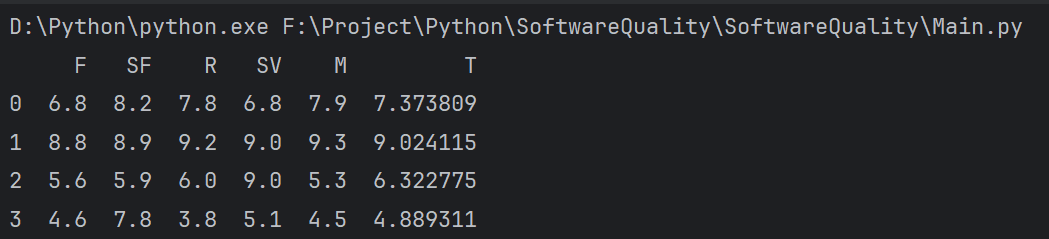
\includegraphics[width=0.5\textwidth]{img5/result.png}
    \caption{软件可信性度量值计算}
    \label{fig:result}
\end{figure}

故最终结果为:

\[
\begin{array}{cccccc}
\toprule
F & SF & R & SV & M & T \\
\midrule
6.8 & 8.2 & 7.8 & 6.8 & 7.9 & 7.373809 \\
8.8 & 8.9 & 9.2 & 9.0 & 9.3 & 9.024115 \\
5.6 & 5.9 & 6.0 & 9.0 & 5.3 & 6.322775 \\
4.6 & 7.8 & 3.8 & 5.1 & 4.5 & 4.889311 \\
\bottomrule
\end{array}
\]

\section{第二道题}

\subsection{题目内容}

有 4 个软件系统,分别编号为 1, 2, 3, 4。它们都有 7 个属性,其中 4 个为关键属性,编号为 $y_1, y_2, y_3, y_4$,其权重分别为 $\alpha_1 = 0.3, \alpha_2 = 0.2, \alpha_3 = 0.35, \alpha_4 = 0.15$。
3 个为非关键属性,编号为 $y_5, y_6, y_7$,其权重分别为 $\beta_1 = 0.35, \beta_2 = 0.40, \beta_3 = 0.25$。

关键属性权重 $\alpha = 0.70$,非关键属性权重 $\beta = 0.30$。根据下表的各属性取值使用模型 $T_3$ 计算各软件的可靠度值。

\begin{table}[H]
\centering
\begin{tabular}{cccccccccc}
\toprule
编号 & $y_1$ & $y_2$ & $y_3$ & $y_4$ & $y_5$ & $y_6$ & $y_7$ & $\varepsilon$ & $\rho$ \\
\midrule
1 & 8.3 & 7.1 & 8.1 & 6.9 & 9.1 & 8.5 & 8.6 & 0.1 & 0.10 \\
  & 7.8 & 8.7 & 8.0 & 6.2 & 8.9 & 8.0 & 8.8 & 0.05 & 0.15 \\
\midrule
2 & 5.8 & 8.1 & 6.8 & 5.6 & 7.9 & 6.8 & 8.1 & 0.1 & 0.10 \\
  & 6.8 & 7.8 & 8.1 & 6.9 & 8.9 & 7.8 & 8.8 & 0.05 & 0.15 \\
\midrule
3 & 3.8 & 3.7 & 4.8 & 4.7 & 3.9 & 5.8 & 6.8 & 0.1 & 0.10 \\
  & 8.4 & 7.2 & 8.1 & 7.7 & 7.9 & 8.8 & 6.8 & 0.05 & 0.15 \\
\midrule
4 & 9.0 & 8.7 & 8.9 & 8.6 & 9.1 & 8.8 & 8.9 & 0.1 & 0.10 \\
  & 8.0 & 7.8 & 6.8 & 8.7 & 7.9 & 8.1 & 8.3 & 0.05 & 0.15 \\
\bottomrule
\end{tabular}
\end{table}

\subsection{题目分析}

根据 \( T_{3} \) 的公式,我们可以逐步写出代码:

先定义各种常数和变量:

\begin{lstlisting} [language = Python, title = { 定义常数和变量 }]
    import pandas as pd
    import numpy as np

    alpha_weights = [0.3, 0.2, 0.35, 0.15]
    beta_weights = [0.35, 0.40, 0.25]
    alpha = 0.70
    beta = 0.30

    data = [
        [8.3, 7.1, 8.1, 6.9, 9.1, 8.5, 8.6, 0.10, 0.10],
        [7.8, 8.7, 8.0, 6.2, 8.9, 8.0, 8.8, 0.05, 0.15],
        [5.8, 8.1, 6.8, 5.6, 7.9, 6.8, 8.1, 0.10, 0.10],
        [6.8, 7.8, 8.1, 6.9, 8.9, 7.8, 8.8, 0.05, 0.15],
        [3.8, 3.7, 4.8, 4.7, 3.9, 5.8, 6.8, 0.10, 0.10],
        [8.4, 7.2, 8.1, 7.7, 7.9, 8.8, 6.8, 0.05, 0.15],
        [9.0, 8.7, 8.9, 8.6, 9.1, 8.8, 8.9, 0.10, 0.10],
        [8.0, 7.8, 6.8, 8.7, 7.9, 8.1, 8.3, 0.05, 0.15] 
    ]

    df = pd.DataFrame(data, columns=['y1', 'y2', 'y3', 'y4', 'y5', 'y6', 'y7', 'epsilon', 'rho'])
\end{lstlisting}

\begin{lstlisting} [language = Python, title = { 获取数据 }]
def calculate_T3(row):
    y_crucial = row[['y1', 'y2', 'y3', 'y4']].values
    y_non_crucial = row[['y5', 'y6', 'y7']].values
    epsilon = row['epsilon']
    rho = row['rho']
\end{lstlisting}

在刚刚的代码的基础上,按照运算顺序计算T3的值:
\begin{lstlisting} [language = Python, title = { 计算 T3 }]
    min = np.min((y_crucial / 10) ** epsilon) # 使用 numpy 自带最小值函数求最小值
    crucial_prod = np.prod(y_crucial ** alpha_weights) # 使用 prod 计算乘积
    crucial_prod_rho = (min * crucial_prod) ** (-rho) # 按照步骤,是 -p 次方
    crucial_value = alpha * crucial_prod_rho # 最后再乘以全局关键属性的权重

    # 有了以上代码,非关键属性的可靠度值也应运而生了。
    non_crucial_prod = np.prod(y_non_crucial ** beta_weights)
    non_crucial_prod_rho = (non_crucial_prod) ** (-rho)
    non_crucial_value = beta * non_crucial_prod_rho

    # 注意,最后的T3值需要用倒数计算
    T_3 = (crucial_value + non_crucial_value) ** (-1/rho)
    return T_3
\end{lstlisting}

\begin{lstlisting} [language = Python, title = {Main 函数}]
    def main():
        df['T3'] = df.apply(calculate_T3, axis=1)
        print(df)

    if __name__ == '__main__':
        main()
\end{lstlisting}

\subsection{题目解答}

\begin{figure} [H]
    \centering
    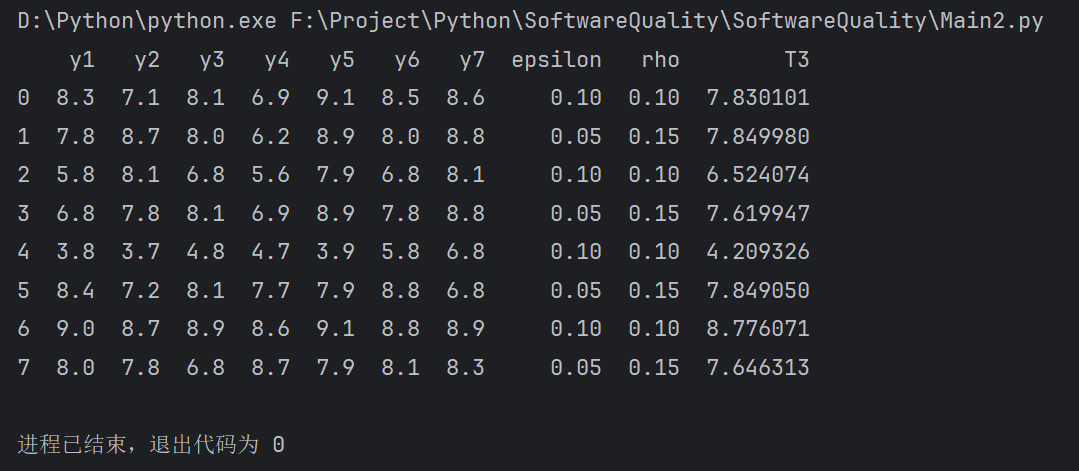
\includegraphics[width=0.5\textwidth]{img5/result2.png}
    \caption{软件可靠度值计算}
    \label{fig:result2}
\end{figure}

\begin{table}[H]
    \centering
    \begin{tabular}{ccccccccccc}
    \toprule
    编号 & $y_1$ & $y_2$ & $y_3$ & $y_4$ & $y_5$ & $y_6$ & $y_7$ & $\varepsilon$ & $\rho$ & $T_3$ \\
    \midrule
    1 & 8.3 & 7.1 & 8.1 & 6.9 & 9.1 & 8.5 & 8.6 & 0.1 & 0.10 & 7.830101 \\
      & 7.8 & 8.7 & 8.0 & 6.2 & 8.9 & 8.0 & 8.8 & 0.05 & 0.15 & 7.849980 \\
    \midrule
    2 & 5.8 & 8.1 & 6.8 & 5.6 & 7.9 & 6.8 & 8.1 & 0.1 & 0.10 & 6.524074 \\
      & 6.8 & 7.8 & 8.1 & 6.9 & 8.9 & 7.8 & 8.8 & 0.05 & 0.15 & 7.619947 \\
    \midrule
    3 & 3.8 & 3.7 & 4.8 & 4.7 & 3.9 & 5.8 & 6.8 & 0.1 & 0.10 & 4.209326 \\
      & 8.4 & 7.2 & 8.1 & 7.7 & 7.9 & 8.8 & 6.8 & 0.05 & 0.15 & 7.849050 \\
    \midrule
    4 & 9.0 & 8.7 & 8.9 & 8.6 & 9.1 & 8.8 & 8.9 & 0.1 & 0.10 & 8.776071 \\
      & 8.0 & 7.8 & 6.8 & 8.7 & 7.9 & 8.1 & 8.3 & 0.05 & 0.15 & 7.646313 \\
    \bottomrule
    \end{tabular}
\end{table}

\section{参考资料}

\begin{itemize}
    \item Pandas官方文档:\href{https://pandas.pydata.org/docs/user_guide/10min.html}{\underline{https://pandas.pydata.org/docs/user\_guide/10min.html}}
\end{itemize}

\end{document}